% ROHC conference for RMLL 2014
%
% The conference is about the ROHC library (https://rohc-lib.org/). It was
% given at [RMLL 2014](https://2014.rmll.info/).
%
% The slides (except the projet and company logos) are Published under the
% CC BY-NC-SA 4.0 license (https://creativecommons.org/licenses/by-nc-sa/4.0/).
%
% Author: Didier Barvaux <didier@rohc-lib.org>

\documentclass[utf8]{beamer}
\mode<presentation>
\title{ROHC: compress your VoIP traffic}
\author[Viveris Technologies]{Didier Barvaux \\ \texttt{didier.barvaux@toulouse.viveris.com} \\ \texttt{didier@rohc-lib.org}}
\date[Formation]{July, 7th 2014}

\usetheme{Warsaw}
%\usecolortheme{whale}
\definecolor{darkblue}{rgb}{0,0,0.8}
\setbeamercolor*{palette primary}{use=structure,fg=white,bg=darkblue}
\setbeamercolor*{palette secondary}{use=structure,fg=white,bg=green!75!orange}
\setbeamercolor*{palette tertiary}{use=structure,fg=white,bg=structure.fg!50!orange}
\setbeamercolor*{palette quaternary}{fg=white,bg=orange}

\setbeamercolor*{sidebar}{use=structure,bg=structure.fg}

\setbeamercolor*{palette sidebar primary}{use=structure,fg=structure.fg!10}
\setbeamercolor*{palette sidebar secondary}{fg=white}
\setbeamercolor*{palette sidebar tertiary}{use=structure,fg=structure.fg!50}
\setbeamercolor*{palette sidebar quaternary}{fg=white}

\setbeamercolor*{titlelike}{parent=palette primary}
\usepackage{ulem}

\begin{document}

% Title
\begin{frame}
		\titlepage
\end{frame}

% Agenda
\begin{frame}
	\frametitle{Agenda}
	\tableofcontents[hideallsubsections]
\end{frame}

% Myself
\begin{frame}
	\frametitle{Me}
	\begin{block}{}
		\begin{columns}
			\begin{column}[T]{85mm}
				\begin{itemize}
					\item 2000-2001: newbie
					\item 2003-2005: diploma from ENSEEIHT
					\item 2005: daily job on Linux at Viveris Technologies {\tiny http://www.viveris.fr/}
					\item 2007: ROHC library {\tiny http://rohc-lib.org/}
					\item 2013: Open Source workgroup at Viveris {\tiny http://opensource.viveris.fr/}
				\end{itemize}
			\end{column}
			\begin{column}[T]{25mm}
				\begin{figure}
					
\includegraphics[height=15mm]{images/viveris_logo.png}
				\end{figure}
				\begin{figure}
					
\includegraphics[height=13mm]{images/rohc_logo.png}
				\end{figure}
			\end{column}
		\end{columns}
	\end{block}
\end{frame}


%%%%%%%%%%%%%%%%%%%%%%%%%%%%%%%%%%%%%%%%%%%%%%%%%%%%%%%%%%%%%%%%%%%%%%%%%%%%%


\section{Header compression}
\frame{\tableofcontents[currentsection,hideothersubsections]}

\subsection{problem statement}
\begin{frame}
	\frametitle{Header compression: why?}
	\begin{block}{Header size}
		Header size is a concern on network links\\
		\pause
		For VoIP traffic, only 20 of 60 bytes for useful data
	\end{block}
	\pause
	\begin{block}{Is header compression still useful?}
		\begin{itemize}
			\item An old idea...
				\begin{itemize}
					\item designed for low-speed serial links in 1990
					\item today network links are much larger
				\end{itemize}
			\item ...but still useful
				\begin{itemize}
					\item slow links still exists (GSM, UMTS...)
					\item larger links are congested
					\item data traffic may be expensive on links (satellite)
				\end{itemize}
		\end{itemize}
	\end{block}
\end{frame}

\subsection{existing protocols}
\begin{frame}
	\frametitle{existing protocols}
	\begin{block}{Protocols defined by the IETF}
		\begin{itemize}
			\item RFC 1144, 1990: Compressing TCP/IP Headers for Low-Speed Serial Links
			\item RFC 2507, 1999: IP Header Compression (IPHC)
			\item RFC 2508, 1999: Compressing IP/UDP/RTP Headers for Low-Speed Serial Links (CRTP)
			\item RFC 3095, 2001: RObust Header Compression (ROHC)
		\end{itemize}
	\end{block}
\end{frame}


%%%%%%%%%%%%%%%%%%%%%%%%%%%%%%%%%%%%%%%%%%%%%%%%%%%%%%%%%%%%%%%%%%%%%%%%%%%%%


\section{The ROHC protocol}
\frame{\tableofcontents[currentsection,hideothersubsections]}

\subsection{definition}
\begin{frame}
	\frametitle{What ROHC is?}
	\begin{block}{RObust Header Compression (ROHC)}
		A network protocol that compresses away protocol headers
	\end{block}
	\pause
	\begin{block}{Objectives}
		\begin{itemize}
			\item efficient \& robust on cellular links
			\item extensible framework {\tiny IPv4, IPv6, UDP, UDP-Lite, RTP, TCP, ESP, GRE...}
		\end{itemize}
	\end{block}
	\pause
	\begin{block}{Standard}
		\begin{itemize}
			\item IETF standard {\tiny http://www.ietf.org/}
			\item ROHC Working Group (WG) {\tiny http://datatracker.ietf.org/wg/rohc/charter/}
			\item RFC 3095 and 22 others
			\item 2 versions: ROHCv1 and ROHCv2
		\end{itemize}
	\end{block}
\end{frame}

\subsection{protocol}
\begin{frame}
	\frametitle{Main principles: headers only}
	Only headers are compressed
	\begin{figure}
		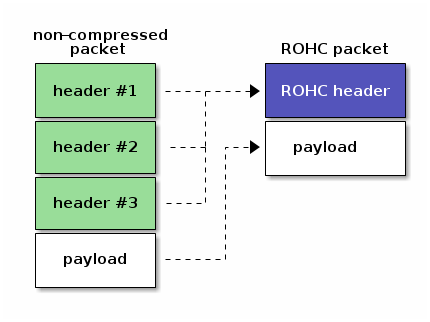
\includegraphics[height=50mm]{images/rohc_only_headers_are_compressed.png}
	\end{figure}
\end{frame}
\begin{frame}
	\frametitle{Main principles: information redundancy}
	Information redundancy:
	\begin{itemize}
		\item within one single network packet, eg. IP/UDP lengths
		\item several network packets in one stream, eg. IP addresses
	\end{itemize}
	\begin{figure}
		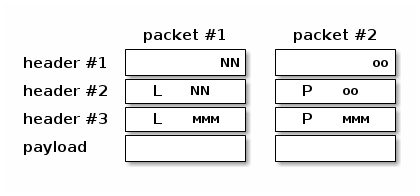
\includegraphics[height=40mm]{images/rohc_redundancy.png}
	\end{figure}
\end{frame}
\begin{frame}
	\frametitle{Main principles: packet classification}
	\begin{figure}
		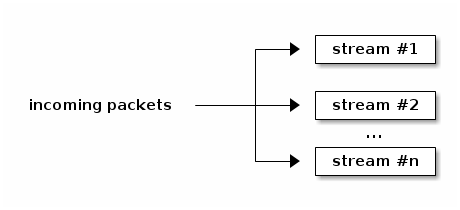
\includegraphics[height=28mm]{images/rohc_classification.png}
	\end{figure}
	\begin{columns}
		\begin{column}[T]{50mm}
			Classify packets into streams: 
			\begin{itemize}
				\item IPv4 / IPv6
				\item IP addresses
				\item UDP/TCP ports
				\item RTP SSRC
				\item ...
			\end{itemize}
		\end{column}
		\begin{column}[T]{50mm}
			Exemples:
			\begin{itemize}
				\item RTP packets of a VoIP call,
				\item TCP packets of a TCP connection...
			\end{itemize}
		\end{column}
	\end{columns}
\end{frame}
\begin{frame}
	\frametitle{Modes of operation}
	Several way to operate:
	\begin{itemize}
		\item the Unidirectional mode (U-mode),
		\item the Bidirectional Optimistic mode (O-mode),
		\item the Bidirectional Reliable mode (R-mode).
	\end{itemize}
	\begin{figure}
		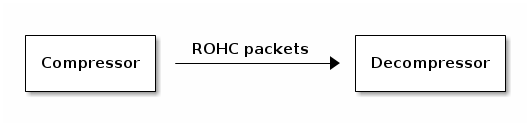
\includegraphics[height=20mm]{images/rohc_umode.png} \\
		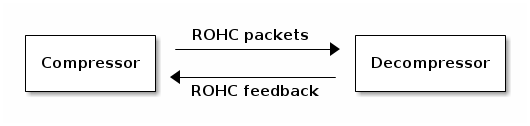
\includegraphics[height=20mm]{images/rohc_omode.png}
	\end{figure}
\end{frame}
\begin{frame}
	\frametitle{Compression states}
	Stateful protocol:
	\begin{itemize}
		\item IR state: low compression, context establishment
		\item FO state: medium compression, transmit small irregular changes
		\item SO state: high compression, transmit only the sequence number
	\end{itemize}
	\begin{figure}
		
\includegraphics[height=15mm]{images/rohc_comp_states.png} \\
		
\includegraphics[height=15mm]{images/rohc_decomp_states.png}
	\end{figure}
\end{frame}
\begin{frame}
	\frametitle{Profiles}
	Compression profiles:
	\begin{itemize}
		\item Uncompressed
		\item IP-only
		\item IP/UDP
		\item IP/UDP-Lite
		\item IP/UDP/RTP
		\item IP/UDP-Lite/RTP
		\item IP/ESP
		\item IP/TCP
	\end{itemize}
	IP = IPv4, IPv4/IPv4, IPv4/IPv6, IPv6, IPv6/IPv4, IPv6/IPv6
	IPv6 extension headers are handled
\end{frame}


%%%%%%%%%%%%%%%%%%%%%%%%%%%%%%%%%%%%%%%%%%%%%%%%%%%%%%%%%%%%%%%%%%%%%%%%%%%%%


\section{The ROHC library}
\frame{\tableofcontents[currentsection,hideothersubsections]}

\subsection{genesis}
\begin{frame}
	\frametitle{Genesis}
	History:
	\begin{itemize}
		\item 2003: initial version by Lulea University of Technologies {\tiny http://www.ltu.se/}
		\item 2007: internal fork by TAS, CNES, and Viveris Technologies
		\item 2009: public version of the fork (GPLv2+)
		\item 2014: LGPLv2+ license
	\end{itemize}
	\pause
	Latest version 1.7.0 released on June 2014:
	\begin{itemize}
		\item ROHCv1 mostly supported
		\item ROHCv2 not supported yet
		\item portable
	\end{itemize}
\end{frame}

\subsection{performances}
\begin{frame}
	\frametitle{Performances}
	30-minute VoIP call\\
	{\tiny 90000 60-byte IPv4/UDP/RTP packets every 20 ms}
	\begin{figure}
		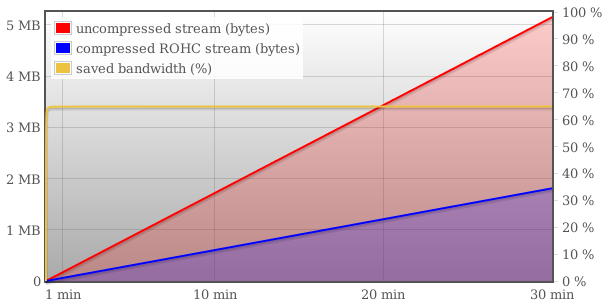
\includegraphics[height=50mm]{images/rohc_perfs.png}
	\end{figure}
\end{frame}

\subsection{applications}
\begin{frame}
	\frametitle{Example}
	\begin{block}{Compressing one IP/UDP/RTP packet}
	\tiny
	struct rohc\_comp *compressor;\\
	...\\
	compressor = rohc\_comp\_new2(ROHC\_SMALL\_CID, ROHC\_SMALL\_CID\_MAX,
	                              gen\_random\_num, NULL);\\
	rohc\_comp\_enable\_profile(compressor, ROHC\_PROFILE\_RTP);\\
	...\\
	rohc\_compress4(compressor, ip\_packet, \&rohc\_packet);\\
	...\\
	rohc\_comp\_free(compressor);\\
	\end{block}
	API documentation, tutorials and examples on http://rohc-lib.org/support/documentation/
\end{frame}
\begin{frame}
	\frametitle{Applications using ROHC}
	\begin{itemize}
		\item tools in sources:
			\begin{itemize}
				\item stats
				\item perf
				\item sniffer
				\item fuzzer
			\end{itemize}
		\item IP/ROHC tunnel (on Launchpad)
		\item OpenSAND {\tiny http://opensand.org/}
		\item used for internal projects by large companies in telecommunications
	\end{itemize}
\end{frame}


%%%%%%%%%%%%%%%%%%%%%%%%%%%%%%%%%%%%%%%%%%%%%%%%%%%%%%%%%%%%%%%%%%%%%%%%%%%%%

\section{Perspectives}
\frame{\tableofcontents[currentsection,hideothersubsections]}

\begin{frame}
	\frametitle{Perspectives}
	\begin{block}{Perspectives}
		\begin{itemize}
			\item new features:
				\begin{itemize}
					\item stable TCP profile,
					\item R-mode
					\item GRE
					\item ROHCv2
				\end{itemize}
			\item better CPU performances
			\item wider usage: SIP phones? IPBX?
		\end{itemize}
	\end{block}
	\begin{block}{Project resources}
	Website: http://rohc-lib.org/\\
	Mailing-list: rohc@lists.launchpad.net\\
	IRC: \#rohc on freenode\\
	\end{block}
\end{frame}


%%%%%%%%%%%%%%%%%%%%%%%%%%%%%%%%%%%%%%%%%%%%%%%%%%%%%%%%%%%%%%%%%%%%%%%%%%%%%

\end{document}

